% !TEX root = ../thesis.tex
% !TeX spellcheck = en_US

As mentioned in the introductory motivation, the developed hybrid routing algorithm has to find optimal paths through open spaces and must also be able to connect arbitrary start and destination locations.
Current routing approaches are either not capable of correctly connecting arbitrary locations (in the case of graph-based algorithm like A*) or do not allow the use of speedup techniques (for example in the \term*{continuous Dijkstra} approach).
Additionally, none of the existing approaches uses both, the open spaces between obstacle and the existing road network, which is still relevant to simulate pedestrian movements.
Edges from a road network often contain useful information, for example about sidewalks, and following roads is therefore a reasonable and realistic routing decision.

The resulting hybrid routing algorithm does not suffer from these disadvantages and therefore offers a fast, flexible and accurate routing.
This chapter covers the design of the implemented algorithm in order to accomplish these tasks.
First, the overall context is presenting specifically the requirements and constraints of the algorithm.
Second, details on the decisions regarding the routing strategy and general design are presented.
Finally, an overview of the separate components is given as well as a description on the deployment of this algorithm.

\section{Requirements and constraints}
	
	Enhancing the routing capabilities of the MARS framework is an integral aspect of the algorithm's development.
	Therefore, the code also uses parts of the MARS framework, which is shown in detail in \Cref{subsec:frameworks-technology}.
	Its design and the resulting architecture, however, are independent of the MARS framework.
	Integrating the algorithm into a different context or using it as a standalone application is therefore possible with minimal changes in the code.
	
	Apart from the integration into MARS, there are several requirements on the algorithm itself, which are presented in the following.
	Technical constraints also exist and are discussed at the end of this section.
	
	\subsection{Requirements}
	
		Functional requirements of the resulting software can be formulated quite easily, since this is not a large commercial product but a single algorithm with a distinct task.
		The hybrid routing algorithm should determine an optimal path between two locations following ways and traversing open spaces while avoiding obstacles.
		A configurable weight function should be used to assign a weight to each edge in order to find the path with the minimum weight.
		Processing of geospatial data must consider existing road network data as well as obstacles, which are features that will be avoided on paths traversing open spaces.
		It must be possible for the shortest path to alternate between segments following roads and open spaces.
		
		More complex and time consuming are the quality requirements.
		Because this is not part of a commercial software development, these requirements are not part of any tender and were not even formulated.
		Nonetheless, they exist and consist of the following aspects.
	
		The largest quality requirement in terms of effort is performance.
		It affects large parts of the software architecture since the resulting algorithm, despite its complexity, should ideally have a negligible impact on the overall performance of a simulation compared to current graph-based routing approaches.
		Routing algorithms and engines often consist of two steps: preprocessing and answering routing queries.
		In order to create fluent and fast simulations, the performance of answering numerous routing requests must be as good as possible.
		The time needed for preprocessing is of less importance.
		
		A rather obvious requirement is the correctness of resulting routes.
		Answers of routing queries must return the shortest route according to a given weight function.
%		Even when using an approximation algorithm to determine shortest paths, the results can be checked against all other possible paths to verify the optimality of the resulting path.
		
		Another quality requirement is the closeness of the resulting routes to real pedestrian behavior.
		Unfortunately, this can hardly be measured without having extensive data of pedestrians and their trajectories in the real world.
		Ideally, the trajectory of a calculated route should be identical to a real-world pedestrian trajectory.
		It should at least make sense to an observer without additional knowledge of the real-world location.
		The coordinates of waypoint on the calculated and on real trajectories must not be exactly the same, since real pedestrian behavior is not part of the shortest path calculations but is instead a task for realistic agent modeling.
		Such behavior includes for example a typical minimum distance kept to obstacles or a minimum radius of walked curves.
	
	\subsection{Constraints}
	\label{subsec:constraints}
		
		% Well integrated into MARS and NTS, no new dependencies
		One major constraint is the integration of final algorithm into the \term*{MARS} framework to make the use as easy as possible and to centralize the code base for better maintenance.
		This means the programming language will be C\# and additionally, because MARS uses the geospatial framework \term{NetTopologySuite} (\term*{NTS}) as basis for all major geospatial operations, this algorithm will be based on NTS.
		However, the higher level architecture and its components is not affected by these technical constraints.
		
		The planned integration into another code base, in this case the one of the MARS framework, affects the management of dependencies.
		On the one hand, the amount newly introduced dependencies should be kept to a minimum, which means dependencies on MARS and NTS are to be preferred over other third-party libraries.
		On the other hand, using only libraries on which MARS depends as well is not always possible due to version mismatches.
		More specific, a triangulation method was needed, which is part of an NTS version not used my MARS yet.
		However, this case only appeared once and can be avoided and should disappear with future dependency updates.
		
		An additional constraints is the limitation on vector data as data structure for obstacles and roads.
		Using raster data is theoretically possible, as mentioned in \Cref{subsection:generate-graphs-from-maps} for the work of Walter et al., but requires a different processing and results in less accurate results, due to the rasterization.
		Therefore, only vector data has to be supported.
	
\section{Combination of routing algorithms}
\label{sec:combining-routing-algorithms}

	This section describes the core aspect of this thesis:
	The decision of a strategy to combine graph and geometric routing algorithms.
	A decision on this \enquote{merge} strategy is crucial to the design and architecture of the application.
	
	The following four approach candidates were considered and are discussed in more details.
	The last of which was considered to be the most promising and was therefore implemented.
	\begin{enumerate}
		\item Ad hoc generation of edges
		\item Concurrent routing
		\item Concurrent routing on smaller segments
		\item Merge an existing network with a visibility graph
	\end{enumerate}
	
	% Ad-hoc creation of edges by stopping A* and continuing with wavefront algorithm
	\subsection{Ad hoc generation of edges}
	
		The idea of an ad hoc generation of edges is the following:
		Whenever the graph routing algorithm reaches a road junction, it's paused and the continuous Dijkstra algorithm is started.
		No destination vertex is defined, which means the geometric routing will be stopped after the furthest wavelet reached a certain distance.
		The continuous Dijkstra approach actually creates a shortest path map, so the shortest paths to all reached vertices are calculated.
		All shortest path edges are then added to the graph for the paused graph-based routing algorithm.
		
		A real-world example for this approach would be a pedestrian walking down a road, stopping at a junction to decide where to go and choosing the option to cross a park for a shortcut before continuing to follow the roads again.
		Doing the shortcut was not planned but an ad hoc decision, just as the algorithm would do.
		
		The advantage of this approach is the realistic behavior of pedestrians not planning the route in beforehand.
		In fact Teknomo and Millonig introduced a routing mechanism for agent-based simulations with the assumption of little to no apriori knowledge of agents about their environment\cite{teknomo-millonig-routing}.
		This approach would therefore implement their assumptions on agents behaviors.
		
		One disadvantage is a relatively high complexity since no standard algorithm from frequently used software frameworks support a pause functionality, so any routing algorithm has to be manually adjusted or implemented from scratch.
		
		Also this approach will likely cause performance issues.
		When using Dijkstra as graph-based routing algorithm, $\bigo{|V|}$ many vertices are visited, which leads to $\bigo{|V|}$ routing requests using the geometric continuous Dijkstra algorithm.
%		Because a simple caching of the shortest path map is not possible, at least not without a smart and complex caching strategy, this decreases the runtime of the whole routing process significantly.
		Even when using the continuous Dijkstra approach from Hershberger and Suri\cite{hershberger-suri} with only $\bigo{n \log n}$ time requirement, the number $n$ of vertices in obstacles is expected to be much higher than the size of $V$ resulting in a somehow quadratic runtime.
		Caching the shortest path map using a \term*{CPD} (see \Cref{subsubsec:cpd}) would be possible but would also increase complexity during query time and reduce performance during preprocessing time.
		Storing precomputed edges in a simple map would reduce complexity, still increase query time but also still reduce precomputation time.
		
		The ad hoc idea of this approach yields no significant advantage compared to a preprocessing.
		Therefore, this approach was not further pursued.
		
%		Another aspect against this approach is the fact that an ad hoc generation of edges will probably not change the resulting shortest path in comparison to a precomputation of these edges.
%		An argumentation for the correctness of this hypothesis can be sketched as follows.
		
%		Assume that the ad hoc generation starts at each road junction vertex $j$ and stops when a certain condition is fulfilled (for example only generating paths of a certain length).
%		When the graph routing algorithm reaches an unvisited junction vertex $j$ from some other vertex $v$, it either used a road edge or preprocessed edge to get there. Therefore, the following two cases exist:
%		\begin{itemize}
%			\item In case a preprocessed edge was used, then the shortest path from $v$ to $j$ would be identical when using a completely preprocessed graph containing this exact edge $(v, j)$.
%			\item In case a road edge was used to get to $j$, then there are two sub-cases.
%			\begin{itemize}
%				\item In case the road edge was in deed the optimal path to $j$, it would have been used in a preprocessed graph as well.
%				\item In case the road edge was not the optimal path, then the ad hoc generation stopped before reaching $j$ (due to the distance or any other stopping condition) and the edge $(v, j)$ was never added.
%			\end{itemize}
%		\end{itemize}
%		Even though this is not a formal proof, generating a preprocessed graph and using a normal routing algorithm is probably as least as good as using the ad hoc generation approach.
	
	% Concurrent routing: Use A* and wavefront in parallel and merge the results
	\subsection{Concurrent routing}
	
		A different approach would be two concurrent routing queries, one on the normal road graph and one using a visibility or otherwise generated graph.
		Having the two shortest paths, they could be merged into one path, which results in segments with alternating source graph.
		To merge them, first the intersection points need to be determined and then the better segments have to be chosen based on a weight function.
		
		The most prominent advantage is the simplicity of the routing requests, since known routing algorithms could be used.
		Therefore, it would be rather simple to implement and speedup techniques could be used.
		
		However, there are two major disadvantages.
		First, it is uncertain that the two paths are actually intersecting at any point.
		Second, even if they are intersecting, too few intersections on a long route result in suboptimal paths, because the longer a segment gets, the less accurate the weighting becomes.
		Only if the two routes are intersecting frequently enough, the selection of segments based on the weight function could actually result in good routes.
	
	% Concurrent routing for segments (e.g. start new routing calls every 100m)
	\subsection{Concurrent routing on smaller segments}
	
		This approach is very similar to the one above, but it tries to fix the uncertainty of intersections between the two resulting paths.
		Multiple ways are conceivable to ensure that there are enough intersections or to otherwise guarantee that segments are small enough to be merged.
		
		One way is to stop the routing after a certain distance stopping at the next available vertex.
		After stopping for the first time, there are two such vertices, one where the road network-based routing stopped and one where the routing on the generated graph stopped.
		From each vertex, two new routing queries start and stop again after a certain distance.
		This continues until one query reaches the destination.
		On the one hand, this would guarantee small enough segments for later merging, on the other hand, this results in $\bigo{2^n}$ many routing queries.
		Even though each query is short, this approach would probably, even with the help of heuristics or other helping mechanisms, not scale very well.
		
		A different approach to obtain smaller segments would be to first get the shortest path on the road graph.
		Having this path, it is split up into $n$ segments of certain length connecting the vertices $v_0, v_1, ..., v_n$ with $v_n$ being the destination.
		In a next step, shortest paths from each vertex to following vertices are calculates.
		Meaning from $v_i$ paths to $v_{i+1}, v_{i+2}, ..., v_n$ are determined, which unfortunately results in $O(n^2)$ many routing queries.
		Finally, all these paths on the generated graph can be merged together with the query result of the road graph to form a new intermediate graph..
		Finally, one last routing query on this intermediate graph is performed to get the final optimal routing result by using a weight function analogous to the previous approach.
		Instead of an intermediate graph, other combinatorial approaches can be used as well since the shortest path problem can be solved using linear programming\cite{handler-zang-lp-duality}.
		
		There are probably more possible ways to ensure a sufficient amount of segments or intersections, however, this idea was not further pursued.
		
		Unfortunately, both approaches have a worse time complexity than any popular routing algorithms including pure geometric routing.
		\todo[inline]{Be more precise}
		Even though the second idea might work well for appropriate segments lengths, the complexity and definite time overhead make it an unfavorable choice.
	
	% Merge of networks
	\subsection{Merge an existing network with a visibility graph}
	
		Previous approach candidates tried to first calculate shortest paths and then merge their results.
		This last approach, which is the currently used one, first merges a generated visibility graph with an existing road graph.
		The actual merge operation is very simple:
		Whenever a road edge and a visibility edge intersect, split the edges, create a new vertex at the intersection point and connect the split edges accordingly.
		
		Even though this approach is simple and still fast, the main disadvantage is the graph size.
		A visibility graph is large and in most cases it will contain many more edges than the road graph, which negatively affects the routing performance.
		
		Another disadvantage is the time complexity of the merge operation.
		All edges have to be considered and, depending on the number of intersections, edges might be processed multiple times (e.g. one visibility edge might intersect with all road edges).
		This leads to at most $|E_R| \cdot |E_V|$ many merge operations for the routing graph edges $E_R$ and visibility edges $E_V$.
		Complete graphs have the highest number of edges and therefore the highest number of intersections, which gives the upper bound of $\bigo{|E|^2}$ for the merge operation given all edges $E$.
		
		Fortunately, road networks are very sparse and often have a vertex degree between three and six\cite{zhao-analysis-osm-bejing}\cite{boeing-osmnx}, resulting in a probably much better runtime behavior in practice.
		The road network of Germany's state North Rhine-Westphalia (NRW) and Hamburg (HH) show the following degrees when analyzing using OpenStreetMap data.
		The state of NRW, which is densely populated and the largest German state in terms of the amount of data, has an average degree of 2.1 but when ignoring dead-ends and touching segments, i.e. when only considering actual junctions, the degree increases to 3.1.
		The state of HH, which is used for the evaluation of this work, has an average degree of 2.11 and 3.11 respectively.
		A vertex with a degree of 10 or higher does not exist in either of these two states.
		\todo[inline]{Link to possible optimizations discussed in later chapters}
		
		Despite the disadvantages of this approach, I considered the advantages to be more important.
		As already mentioned, this strategy is not only simple and fast, it also allows the use of speedup methods for routing queries, e.g. the A*-based ALT algorithm or other techniques described in \Cref{subsec:speedup-methods}.
		Moreover, the resulting path is definitely optimal, based on the given weight function, and no complex postprocessing is needed.
		Such postprocessing is, for example, needed in the \enquote{concurrent routing} candidate approach.
		
		Taken all aspects into account, this strategy seemed to be the simplest and most promising with the least disadvantages.
		It was therefore chosen to be implemented.

\section{Design decisions}
\label{sec:design-decisions}

	With the choice of the strategy to combine graph-based and geometric routing, several design decisions were made.
	Some decisions did not influence the overall architecture and were just made to enhance performance or simplify the implementation.
	Therefore, this section covers fundamental decisions relevant for the overall architecture only.
	\Cref{chap:implementation} covers those decisions that are independent of the overall architecture.
	
	In this work I implemented the visibility graph without the use of algorithms presented in the according \hyperref[subsec:related-work:visibility-graph]{related work section}.
	None of the existing approach would have been easy to implement without problems.
	Details on these problems and the exact reasons that led to the decision of a custom implementation are presented in this section as well.
	
	\subsection{Requirements and considerations for the visibility graph creation}
	
		One key requirement for the visibility graph creation is the ability to work in arbitrary obstacles, which primarily includes the fundamental point, linestring and polygon geometries.
		To work with arbitrary real-world datasets, assumptions about the collinearity, position of obstacles and intersections between them cannot be made.
		
		An important special case arises for linestring obstacles consisting of more than two points.
		Simply determining visibility edges to and from both sides of the linestring would result in shortest paths leading right through it.
		This is the opposite of the desired behavior of a shortest path leading \emph{around} the linestring obstacle.
		The same situation would arise with two arbitrary obstacles, including polygonal ones, touching each other in a single vertex.
		
		Since the visibility graph is solely used to determine shortest paths, some assumptions and optimizations can still be made.
		As mentioned above, these optimizations did not influence the overall architecture and are therefore described in detail in \Cref{sec:visibility-graph-creation}.
		
		A core aspect of the routing algorithm is the reachability of arbitrary locations not located on the graph.
		Adding visibility edges after the complete graph has been created must therefore be possible.
		Implementing this is necessary regardless of the chosen algorithm for the visibility graph creation.
		
		As the generation of the routing graph happens in a preprocessing step, the time and space needed for this task was not a critical aspect of the whole algorithm.
		Further optimizations are possible and discussed in \todo[inline]{link to future work}.
		Significant to agent-based simulations is the routing behavior itself as it directly affects the simulation time.
		Creating the graph in a preprocessing step has, especially when persisting the graph for multiple uses, no direct effect on the simulation.
		
		All these requirements and considerations, including problems and efforts outlined below, lead to the decision of implementing a simple graph generation approach with some easy but effective optimizations.
	
	\subsection{Suitability of existing approaches}

		The largest and most influential design decision was the decision against an approach from the literature as presented in \Cref{subsec:related-work:visibility-graph}.
		Several approaches from the literature have either restrictions on the geometric structures or assume that a certain preprocessing of the data was already performed.
		
		The approach by Welzl\cite{welzl-visibility-graph}, for example, explicitly assumes that there are not collinear vertices, i.e. at least three vertices forming a straight line.
		It may seem unlikely at first that collinear vertices occur in real-world datasets, but in fact, at least in OpenStreetMap, it is very common to align touching buildings and other straight obstacles like walls.
		\todo[inline]{diagrams/graphics for problems like this alignment thing}
		
		An optimization of Welzls approach, by Overmars and Welzl\cite{overmars-weizl-visibility-graph}, only works on non-intersecting line segments.
		Real-world data is unfortunately too diverse to fulfill this criterion as polygons, longer linestrings and other more complex data structures exist.
		Preprocessing the data, i.e. cutting all geometries into such non-intersecting line segments, would cause new special cases to solve.
		For example, cutting a polygon into line segments would add visibility edges within the former polygon, which needs to be avoided e.g. by storing metadata about the relations of these line segment to each other.
		Handling all those special cases, preventing unwanted edges and still using the approach by Overmars and Welzl would be possible but would also increase the complexity of their approach.
		
		Another approach with the limitation of no collinear vertices was the plain-sweep algorithm by Ghosh and Mount\cite{ghosh-output-sensitive-vgraph}.
		In addition to the limitation on collinear vertices, they assume x-coordinates to be unique, which would need to be handled as well.
		Even though coordinates are usually floating point numbers and therefore have a great range of possible values, rounding and size limitations reduce this range and might result in a high number of non-unique x-coordinate values.
		Counting the number of non-unique x-coordinates in OpenStreetMap illustrates this problem:
		The OSM dataset of the German state of Hamburg contains over 3.2 million nodes of which 22.8\% have a non-unique x-coordinate.
		
		Kapoor and Maheshwari presented a visibility graph creation as well\cite{kapoor-shortest-path-vgraph} but assumed a triangulation of the open space between the obstacles.
		Such a triangulation can be done quite fast, algorithms with time complexities of $\bigo{n \log{n}}$ and better are known\cite[58-60]{de-berg-computational-geometry}, but libraries such as MARS or the NetTopologySuite do not implement this.
		They only provide triangulation methods for polygons but not for the space between them.
		Implementing an algorithm for this task would be needed in addition to the visibility graph creation itself.
		
		Probably all approaches from the literature would work but preprocessing, restrictions on the input data or adjustments to the approaches would be necessary.
		Since this work focuses more on the overall concept of a hybrid routing algorithm, the choice on the graph generation algorithm was of less importance.
		Therefore, the implementation in this work, as shown in \Cref{chap:implementation} in detail, is much simpler and independent of the aforementioned approaches.
		
	\subsection{Early implementation based on the continuous dijkstra paradigm}
		
		An early implementation, before the above mentioned decision for a strategy fell, was not creating a visibility graph but instead it was based on the \term*{continuous dijkstra} paradigm with wavelets propagating through open spaces.
		However, there were three reasons why this first approach was replaced by a visibility graph-based algorithm.
		
		The main reason was the overall strategy decision on the visibility graph approach.
		One other reason was the implementation of performance enhancement for the naive continuous dijkstra.
		Early stages of the continuous dijsktra approach used a very naive and simple implementation without optimizations mentioned in recent literature on this topic.
		Wavelets did not move continuously but instead they snapped to the next \enquote{event}, i.e. to the next visible vertex where new wavelets can spawn.
		Because the strategy decision was not yet made at that time, no larger efforts went into optimizing the implementation, e.g. by implementing the approach presented by Hershberger and Suri\cite{hershberger-suri}.
		Instead, a simple preprocessing was introduced and lead to a major performance improvement.
		This preprocessing determined the visibility between all vertices used for the above mentioned events.
		Such predetermined visibilities are the core idea of a visibility graph, thus moving to an approach using an actual visibility graph was only a small step.
		
		A third reason against this early continuous dijkstra implementation were the difficulties and the disadvantages of combining the network-based routing with the continuous dijkstra algorithm, as described in \Cref{sec:combining-routing-algorithms}.
		
		Therefore, this first continuous dijkstra approach was not further pursued but converted to a generator for a routable visibility graph with components described in the following section.
	
\section{Components}
\label{sec:components}

	The hybrid routing algorithm consists of two main components, which present public interfaces.
	Generating the underlying routing graph, the so-called \term{hybrid visibility graph}, is the first step and resides in its own component, the \texttt{HybridVisibilityGraphGenerator} class.
	The hybrid visibility graph itself is contained in the \texttt{HybridVisibilityGraph} class, which primarily contains the graph structure and is used to answer routing queries.
	A third component, which is not intended to be used from outside the algorithm, is the \texttt{VisibilityGraphGenerator}.
	Its purpose is the determination of visibility edges for the routable hybrid visibility graph.
	
	Since this works resides in a rather technical and algorithmically oriented context, there are no other components involved, like for example a user interface.
	Also, there are no independent services or applications communicating with or depending on each other, as it would appear in a microservice architecture with different services like an HTTP proxy, application servers and a database.
	
	\begin{figure}[h]
		\begin{figcenter}
			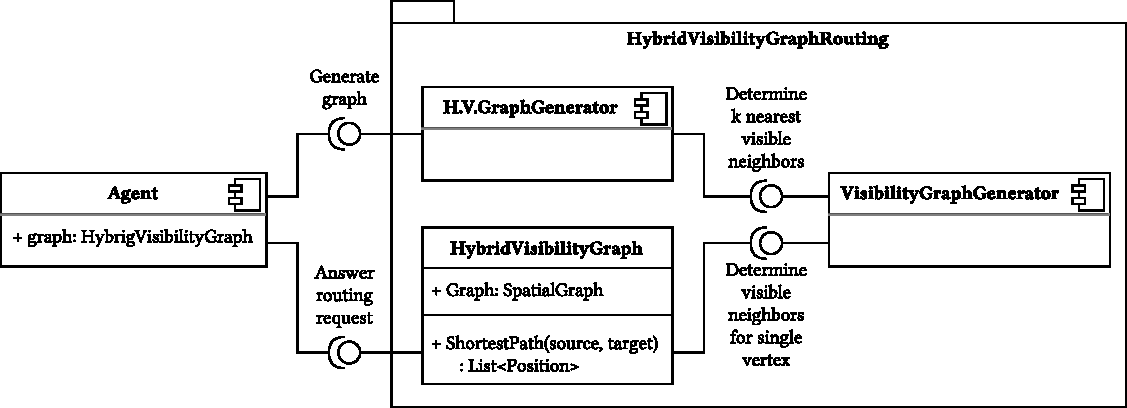
\includegraphics[width=\textwidth]{images/components.pdf}
		\end{figcenter}
		\caption{The components and usages of interfaces of the resulting implementation.}
		\label{fig:components}
	\end{figure}
	
	In an agent-based simulation, each agent has the ability to make its own decisions, which includes the calculation of routes as part of its path planning routing.
	The hybrid visibility graph has the necessary interfaces to answer routing queries, which means, an agent needs access to an instance of this graph for its navigation.
	In \Cref{fig:components}, the agent itself creates this graph but the visibility graph can also be shared among multiple agent and therefore does not need to be created multiple times for the same input dataset.
	
	The \texttt{HybridVisibilityGraphGenerator} (abbreviated as \enquote{H.V.GraphGenerator} in \Cref{fig:components}) presents a public \texttt{Generate()} method for the task of the graph generation and, in this exemplary setup, is used by the agent.
	It returns an instance of the \texttt{HybridVisibilityGraph} class offering public methods to answer shortest path queries.
	These methods, such as \texttt{OptimalPath(source, destination, weightFunction)}, then return a list of coordinates representing the shortest path between two input coordinates.
%	More details on the graph generation can be found in \Cref{sec:graph-generation}.
	
%	For convenience and due to required preparations, routing queries are put to the hybrid visibility graph.
	To fulfill the overall concept of this work, it must be possible to start and end at arbitrary locations, thus, there is no guarantee that the source and destination locations of the query are on any vertex in the graph.
	Therefore, the hybrid visibility graph has to temporarily connect these locations to the graph.
	This is done by determining all visible neighbors of the source and destination locations and merging the resulting edges to the underlying graph.
	To perform this task, the hybrid visibility graph uses the interface of the \texttt{VisibilityGraphGenerator} to determine visibility neighbors of a single vertex.
	In other words, it utilizes the central step of the graph generation process to connect the two input coordinates.
	\Cref{sec:answering-queries} covers the process of answering routing queries in more details, including a clean up step that is performed after the shortest path has been found.

\section{Deployment view}

	% published in MARS
	\todo{Publishing in MARS}

